\chapter{Użyte narzędzia i technologie}\label{chap:technologie}

\section{Język programowania}\label{sec:jezyk_programowania}

Glasgow Haskell Compiler został napisany w języku Haskell. Wykorzystano została w projekcie technika \foreign{bootstraping}, polegająca na tym, iż kompilator rozwijany jest w języku, który kompiluje i jedną z zależności potrzebną do zbudowania GHC jest on sam. Środowiskiem wykorzystanym do edycji kodu było IntelliJ IDEA z wtyczką zapewniającą wsparcie dla języka Haskell. Wtyczka ta niestety w pełni działa tylko z projektami systemu Cabal i nie jest dostosowana do prac nad GHC. Z tego powodu środowisko nie zapewniało na przykład ciągłego raportowania błędów w kodzie lub wyszukiwania deklaracji określonego typu, choć z tych udogodnień można korzystać w innych projektach.

Drugim językiem wykorzystanym w GHC jest Python. Testowanie i walidacja kompilatora są realizowane przez skrypty w tym języku, więc dodając nowe testy w pracy należało się z nim zetknąć. kontakt. Jest on wymagany do zbudowania GHC również z tego powodu, że do stworzenia dokumentacji wykorzystane zostało narzędzie Sphinx wymagające interpretera.

W projekcie użyty został również język C do napisania środowiska uruchomieniowego, linkowanego z każdym programem skompilowanym przez GHC. W pozostałych częściach GHC można znaleźć dyrektywy preprocesora C, który GHC może wykorzystać zanim przejdzie do kompilacji. W tej pracy jednak kontakt z nim był znikomy.

\section{Narzędzia}

\subsection{Git}

Kod GHC znajduje się w repozytorium Git i jest publicznie dostępny do pobrania. Biblioteki wykorzystywane w kompilatorze również są przechowywane w repozytoriach Gita, lecz są osobnymi projektami, dołączonymi do GHC jako submoduły. Klon oficjalneago repozytorium znajduje się również w popularnym serwisie GitHub. Prawa zapisu do repozytorium są ograniczone\cite{WikiGettingTheSources}.

Krokiem wymaganym do rozpoczęcia pracy było sklonowanie repozytorium i lokalne zbudowanie kompilatora ze źródeł. Po lokalnej edycji plików zmiany musiały zostać zapisane w repozytorium i opatrzone komentarzem stosującym się do konwencji opisanej na wiki GHC, zanim mogły zostać wysłane z użyciem systemu Phabricator.

\subsection{Trac}

Trac to system do organizacji pracy programistów. Przechowuje listę zgłoszeń, czyli spójnych propozycji zmian w projekcie. Zapisywane są w nim zadania do wykonania oraz błędy wykryte w GHC, także przez zwykłych użytkowników. Chroni to je przed zapomnieniem w razie, gdyby nie istniała możliwość zajęcia się nimi od razu. Znajdują się w tym systemie również propozycje dodania nowych funkcji. Do każdego zgłoszenia może być dołączony opis, w przypadku błędu sposób reprodukcji, zapewnione jest miejsce na dyskusję i mechanizm śledzenia stanu wykonania zadania. Aby ułatwić organizację pracy, do zgłoszeń możliwe jest przypisanie właściciela, by zapobiec sytuacji, w której jedną rzecz wykonuje wiele osób. Możliwe jest określenie priorytetu i planowanej wersji, w której zadanie powinno już być wykonane i późniejsze sprawdzanie, czy ten cel został osiągnięty. Ułatwione jest również umieszczanie odnośników do innych, powiązanych zgłoszeń czy do systemu Phabricator. Wszystkie te funkcje wykorzystywane są w GHC.

\begin{figure}[ht]
    \centering
    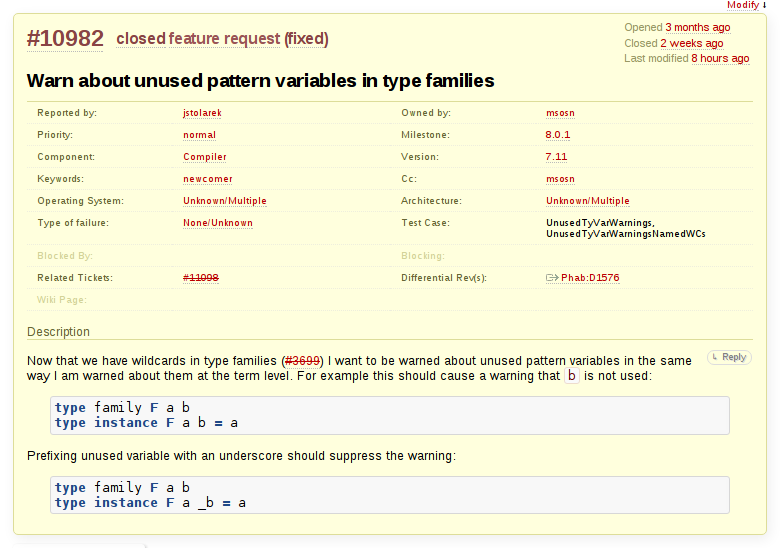
\includegraphics[width=0.8\textwidth]{images/Trac_description}
    \caption{Opis zgłoszenia w systemie Trac}
    \label{fig:Trac_description}
\end{figure}

Przykład zgłoszenia widoczny jest na rysunku \ref{fig:Trac_description}. Dotyczy ono jednego z wykonanych w pracy usprawnień, pozostałe również mają swoje opisy w systemie. Aktualizacja informacji na stronie Trac jest wymagana przez procedurę wprowadzania zmian w GHC\cite{WikiFixingBugs}.

\subsection{Phabricator}

\cite{WikiPhabricator}

Phabricator wykorzystywany jest do inspekcji kodu w czasie zgłaszania ulepszenia oraz do automatycznej walidacji z wykorzystaniem narzędzia Harbormaster. Inspekcja jest ułatwiona, gdyż program prezentuje obok siebie wersję sprzed i po dokonaniu zmian, z wyróżnieniem zmodyfikowanych linii kodu. Daje też możliwość komentowania wybranych fragmentów.

\begin{figure}[ht]
    \centering
    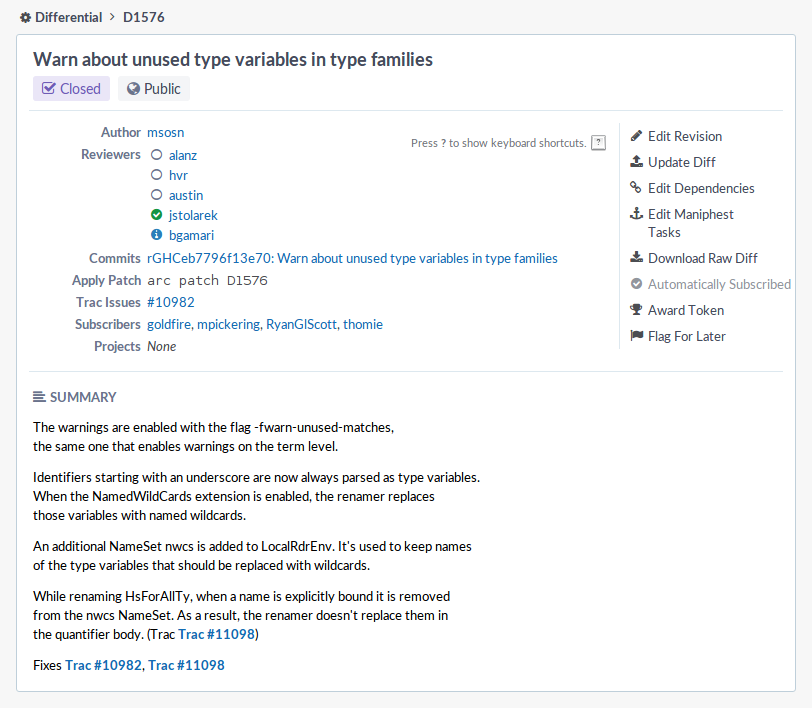
\includegraphics[width=0.8\textwidth]{images/Phabricator_summary}
    \caption{Informacje o proponowanej zmianie w kodzie na stronie Phabricator}
    \label{fig:Phabricator_summary}
\end{figure}

Na rysunku \ref{fig:Phabricator_summary} widać opis jednego z ulepszeń dokonanego w tej pracy. Zgodnie z procedurą \cite{WikiFixingBugs}, aby zmiany zapisane w lokalnym repozytorium Git znalazły się na serwerze, łatka musi przejść wpierw przez proces rewizji w systemie Phabricator. Polega on na tym, iż inni programiści, szczególnie ci, którzy posiadają uprawnienia do zapisu do repozytorium, zapoznają się z przesłanym kodem. Zgłaszają oni swoje uwagi i decydują, czy zmiana może zostać naniesiona na repozytorium na serwerze, czy wymaga poprawek.

\begin{figure}[ht]
    \centering
    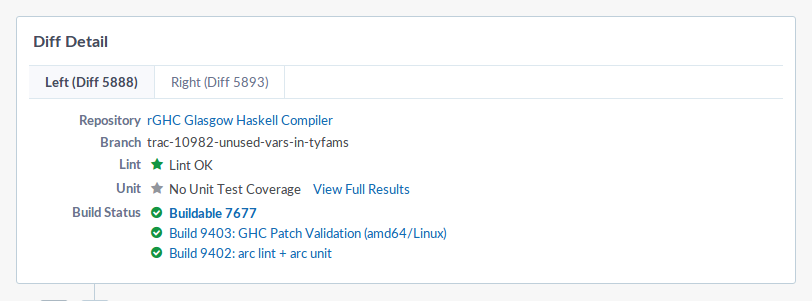
\includegraphics[width=0.9\textwidth]{images/Phabricator_validate}
    \caption{Wynik walidacji programu Harbormaster widoczny na stronie Phabricator}
    \label{fig:Phabricator_validate}
\end{figure}

Z chwilą wysłania proponowanych zmian w kodzie do Phabricatora, wykonane zostaje również automatyczne zbudowanie i przetestowanie nowej wersji GHC przez moduł Harbormaster na przeznaczonym do tego serwerze. Jeżeli walidacja wykryje błędy, jest to znak, iż konieczne są poprawki i oszczędza to czas poświęcony na inspekcję kodu przez programistów. Na rysunku \ref{fig:Phabricator_validate} widać raport z Harbormastera do jednego z wprowadzonych w tej pracy usprawnień, w którym nie wykryto problemów.

Jak wspomniane zostało w sekcji \ref{sec:jezyk_programowania}, GHC jest budowany z użyciem innej wersji GHC. Aby zapewnić stabilność, istnieje wymaganie, że nowa wersja kompilatora musi być możliwa do skompilowania z wykorzystaniem jednej z dwóch poprzednich stabilnych wersji\cite{WikiFixingBugs}. Sam proces budowania przebiega wieloetapowo. Najpierw, z użyciem starszej wersji kompilatora, budowane są biblioteki, zależności GHC. Następnie kompilowany w ten sposób jest sam GHC, czego rezultatem jest kompilator w nowszej wersji. Następnie te dwa kroki, budowania bibliotek i kompilacji GHC, są powtarzane, lecz z wykorzystaniem nowego kompilatora i to on jest uznawany za wynik całego procesu\cite{WikiBuildSystem}. Dzięki temu sposobowi działania, usprawnienia w kompilacji są od razu zastosowane do kompilatora, przy jednym etapie wykorzystywane byłyby optymalizacje i sposób generowania kodu ze starszej wersji. Stanowi to również dobry test nowej wersji, gdyż jeżeli pojawiły się w niej nowe błędy, to jest duża szansa, iż ujawnią się one w czasie budowania kompilatora na drugim etapie.

Uzyskany kompilator jest poddawany kilku tysiącom testów. W większości dzielą się one na trzy kategorie: testów, w których kompilacja pewnego programu musi zakończyć się powodzeniem; testów, których kompilacja musi zakończyć się błędem; testów, w których kompilacja musi się udać, a następnie sprawdzane jest zachowanie programu po uruchomieniu. Wiele testów polega na sprawdzeniu komunikatów kompilatora i porównaniu ze wzorcem.
